\documentclass[a4paper,12pt]{article}
\usepackage[margin=0.7in]{geometry}
\usepackage[latin1]{inputenc}
\usepackage[english]{babel}
\usepackage{amsmath}
\usepackage{cases}
\usepackage[makeroom]{cancel}
\usepackage{amsmath,tabu}
\usepackage[fleqn]{mathtools}
\usepackage[fleqn]{amsmath}
\usepackage{bm}
\usepackage{tikz}
\usepackage{enumitem}
\usepackage{wrapfig}
\usepackage{graphicx}
\usepackage{siunitx}
\usepackage{microtype}
\usepackage{array,tabularx}
\usepackage{float}
\usepackage{booktabs}
\usepackage{import}
\usepackage{cases}
\usepackage{myUnitOfMeasure}
\usepackage{myThermodynamics}
\usepackage{myMath}

\title{PRECEPT 6: Environmental impact of a power plants}
\author{Rossi Andrea 875272}
\date{}


%\newcommand{\pointdatatable}[5]{
%\begin{center}
%\tabulinesep=1.2mm
%\begin{tabu}{|l|c|c|c|}
%\hline
%$ T_{#1} $ & $ p_{#1} $ & $ h_{#1} $ & $ s_{#1} $\\ \hline
%$ \round{#2} \celsius $ & $ \round{#3} \,bar $ & $ \round{#4} \kjkg $ & $ \round[round-precision=4]{#5} \kjkgk $\\ \hline
%\end{tabu}
%\end{center}
%}

%\newcommand{\Lt}{L_{tubes}}
\newcommand{\Lt}[1][\,]{L^{#1}_{\text{tubes}}}
\newcommand{\It}[1][\,]{I^{#1}_{\text{tubes}}}
\newcommand{\Nt}[1][\,]{N^{#1}_{\text{tubes per row}}}
\newcommand{\Nr}[1][\,]{N^{#1}_{\text{rows}}}
\newcommand{\Tcond}{T_{\text{cond}}}
\newcommand{\Tevap}{T_{\text{evap}}}
\newcommand{\pcond}{p_{\text{cond}}}
\newcommand{\pevap}{p_{\text{evap}}}
\newcommand{\psep}{p_{\text{sep}}}

\newcommand{\coefA}{\round[round-precision=4]{1.207157069183}}
\newcommand{\coefB}{\round[round-precision=4]{1.008756026720797}}

\newcommand{\coefAcoal}{\round[round-precision=4]{1.092675258663658}}
\newcommand{\coefBcoal}{\round[round-precision=4]{0.925692101342649}}
\newcommand{\coefC}{\round[round-precision=4]{0.025063536063922}}
\newcommand{\coefD}{\round[round-precision=4]{1.002541442556882}}

\newcommand{\fgs}{\text{FG+S}}
\newcommand{\dfg}{\text{DFG}}
\newcommand{\fg}{\text{FG}}
\newcommand{\norm}{\text{NORM}}
\newcommand{\dil}{\text{diluter}}
\newcommand{\mgnmcube}[2]{\frac{\mg_{#1}}{\text{Nm}^3_{#2}}}


\newcommand{\cacooo}{\text{CaCO}_3}

\renewcommand{\thesection}{\Alph{section}}
\renewcommand{\thesubsection}{\thesection.\arabic{subsection}}

%
%
%
%
%
%
%
%
%
%
%
\begin{document}
\maketitle

The	object of the precept is to	analyse	the	environmental performance of the steam cycle, whose flue gas composition and mass balances were computed in precept 1.
We must analyse the emissions for two different type of fuel:
\begin{enumerate}[label=\Alph*)]
\item NATURAL GAS
	\begin{itemize}
	\item Concentration of $\nox$ in \emph{dry} flue gases at the stack equal to 45 ppmvd at 3\% of $\oo$ .
	\end{itemize}
\item COAL
	\begin{itemize}
	\item Concentration of $\nox$ in \emph{dry} flue gases at the stack equal to 90 ppmvd at 6\% of $\oo$;
	\item Desulfurizer efficiency $\eta_{\text{desulfurizer}} = \eta_{\soo}= 97.5\perc$
	\end{itemize}
\end{enumerate}
%
For both plants A and B it is required to evaluate:
\begin{enumerate}
\item absolute emission of nitrogen oxides $\nox$ in $\kgs$ as equivalent $\noo$;
\item $\nox$ mass concentration in dry flue gases;
\item absolute emission of $\coo$ in $\kgs$;
\item ONLY for case B, check that concentration in flue gases of $\soo$ respect the legal limit of $200\mg/Mn_3$ with $6\perc$ of $\oo$.
\end{enumerate}
Moreover it is required to compare the emission of $\nox$ and $\coo$ with that produced by a \emph{natural gas combined cycle} plant with the following data:
\begin{itemize}
\item net electric power = $390\mw$
\item LHV efficiency = $0.57\perc$
\item flue gases mass flow rate = $650\kgs$
\item $\nox$ concentration in dry flue gases = $14$ ppmvd at $15\perc$ of $\oo$.
\end{itemize}

\section{NATURAL GAS}
From precept number 1 we have the following concentrations in flue gases;

\subimport{tables/}{flue_gases_methane}

\subsection*{The theoretical model}
Both	in	case	of	use	of	natural	gas	and	coal,	the	text	gives	the	fraction	of	$\nox$	($\no$	and	$\noo$)	at	the	stack.	The	concentration	of	$\nox$	in	ppmvd	is	referred	to	a	certain	\%	of	oxygen	in	the	dry	flue	gases.	This	means	that	the	information	regarding	$\nox$	does	not	correspond	to	the	real	conditions	of	this	pollutant	in	the	flue	gases,	since	the	flue	gases	are	humid	and,	a	priori,	with	a	different	$\perc$	of	oxygen.	

The	legislation	regulating	the	emissions	from	combustion	power	plants	requires,	for	statistical	elaborations	and	technical	comparisons,	that	the	flue	gases	flow	is	expressed	on	a	dry	basis,	i.e.	(virtually)	purged	of	the	humidity	content,	and	normalized	on	a	certain	reference	oxygen	content,	depending	on	the	combustion	system	(The	value	chosen	is	usually	close	to	the	actual	average	value).
%
\begin{figure}[H]
	\centering
    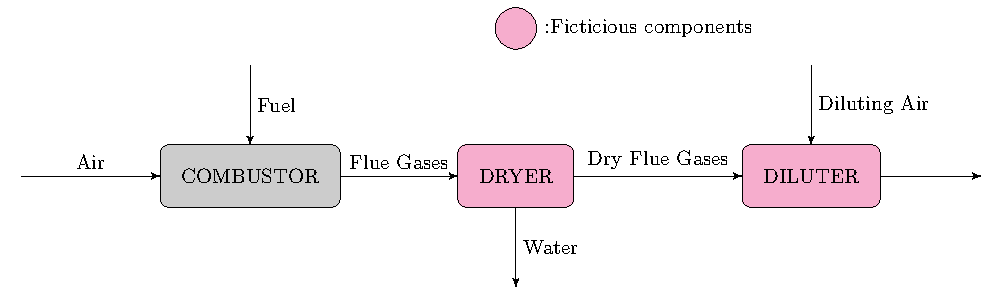
\includegraphics[scale=1]{schemeA.pdf}
    \caption{Scheme of the theoretical model.}
\end{figure}
%
These	two	corrections	(dry	flue	gases	and	oxygen \%)	are	applied	in	order	to	evaluate	concentrations	regardless	of	the	random	effects	affecting	the	combustion	process,	such	as:
\begin{itemize}
\item The	excess	air	in	the	combustor.	The	plant	control	system	acts	on	the	inlet	mass	flow	rate	so	that	the	oxygen	is	kept	at	a	constant	value	in	the	flue	gases.	Nevertheless,	because	of	changes	in	the	chemical	composition	of	the	fuel,	variations	of	load,	etc...	the	oxygen	content	in	the	flue	gases	fluctuates	over	time;
\item Condensation	of	water	in	the	flue	gases.	In	some	processes	(e.g.	condensing	boilers)	water	condenses	reducing	the	flue	gases	mass	flow	rate	at	the	stack.	This	would	turn	out	in	higher	pollutant	concentrations	at	the	stack;
\item Weather	conditions.	The	mass	flow	rate	of	the	combustion	air	inlet	changes	with	air	moisture.
\end{itemize}
Moreover, if the legislation would provide the limits for the pollutants without stating the reference oxygen content and the humidity = 0 in the flue gases, in order to comply with the limit it would be sufficient to dilute the flue gases with ambient air or steam.  

Finally, the flue gases must be brought to normal reference conditions, as the gas density changes with the temperature and pressure. At these conditions (273.15 K and 101325 Pa) 1 kmol of gas occupies 22.414 $m^3$ ($Nm^3$).  
In order to derive the formula that expresses the relation between the actual concentration and the normalized concentration we assume a plant scheme with two fictitious components, defined \emph{diluter} and \emph{dryer}, respectively.  

In a \emph{real plant} there is no dilution of flue gases with ambient dry air (besides some eventual uncontrolled infiltrations of air in the depressed flue gases line), neither any drying.  

From the \emph{mass and concentration balance} between each section we can get a way to pass from one convention to the others for a generic molecule.

\subparagraph*{From FLUE GASES to DRY FLUE GASES}
\begin{equation}
\label{eq:FG_DFG}
\chi_i^{\dfg} = \chi_i^{\fg} \cdot \frac{1}{1 - \chi_{\hoo}^{\fg}}
\end{equation}
where the coefficient $\displaystyle \frac{1}{1 - \chi_{\hoo}^{\fg}}$ is constant and equals to $\coefA$

\subparagraph*{From DRY FLUE GASES to NORMALIZED FLUE GASES}
\begin{equation}
\label{eq:DFG_NORM}
\chi_i^{\norm} = \chi_i^{\dfg} \cdot \frac{\chi_{\oo}^{\norm} - \chi_{\hoo}^{\dil}}{\chi_{\oo}^{\dfg} - \chi_{\oo}^{\dil}}
\end{equation}
We just miss $\chi_{\oo}^{\dfg}$ but we can get it with equation \ref{eq:FG_DFG} applied for the oxygen:
\begin{equation}
\chi_{\oo}^{\dfg} = \chi_{\oo}^{\fg} / \coefA = \round{0.031536364282867*100}\perc
\end{equation}
%
The coefficient $\displaystyle \frac{\chi_{\oo}^{\norm} - \chi_{\hoo}^{\dil}}{\chi_{\oo}^{\dfg} - \chi_{\oo}^{\dil}}$ now can be calculated and it constant and equals to $\coefB$.\\
The diluter is simply ambient air, with an oxygen concentration of $20.7\perc$.

\subsection{Absolute emission of $\nox$ as equivalent $\noo$}
We know the concentration of $\nox$ in dry flue gases with 3\% of $\oo$ so reverting equation \ref{eq:DFG_NORM} we can get the concentration of $\nox$ in dry flue gases. From this value, using equation \ref{eq:FG_DFG} we obtain their absolute concentration in original flue gases.

\begin{align}
\chi_{\noo}^{\fg}  &= (1 - \chi_{\hoo}^{\fg}) \cdot \chi_{\noo}^{\dfg} \\
				   &= (1 - \chi_{\hoo}^{\fg}) \cdot \frac{\chi_{\oo}^{\dfg} - \chi_{\oo}^{\dil}}
{\chi_{\oo}^{\norm} - \chi_{\hoo}^{\dil}} \cdot \chi_{\noo}^{\norm} \\
				   &= \dfrac{45\text{ ppmvd}}{ \coefA \cdot \coefB} 
= \round{3.70037527665980e-05*1000000}\E{-6}
\end{align}
The absolute emission of $\nox$ is computed as:
\begin{equation}
\label{eq:abs_emission}
E_{i} \left[ \kgs \right] = \chi_i^{\fg} \cdot \MM{i} \cdot \ndot{\fg}
\end{equation}
From precept 1 we know that the mass flow rate of flue gases is $\round{4.453413133502107e+02} \kgs$ and their mean molar mass is $\round{27.846123335541750}\kgkmols$. From these values we can evaluate the molar flow rate of flue gases as 
\begin{equation}
\ndot{\fg} = \frac{\mdot{\fg} }{ \MM{\fg}} = \round{15.992937615908412}\kmolss
\end{equation}
We are now able to compute the absolute emission of $\noo$.
\begin{equation}
E_{\noo} \left[ \kgs \right] = \chi_{\noo}^{\fg} \cdot \MM{\noo} \cdot \ndot{\fg}
= \round{0.0272258771724928*1000}\E{-3} \kgs
\end{equation}

\subsection{$\nox$ mass concentration in dry flue gases}
With the conversion coefficient between flue gases and dry flue gases it is not so difficult to evaluate the concentration of $\noo$ in dry flue gases.
\begin{equation}
C_{\nox}^{\dfg} = \dfrac{\cancel{\ndot{\dfg}} \cdot \chi_{\noo}^{\dfg} \cdot \MM{\noo} \E{6} \mg / \kg }{\cancel{\ndot{\dfg}} \cdot 22.414}
= \round{91.5619157547273} \left[ \frac{\mg_{\noo}}{Nm^3_{\dfg}} \right]
\end{equation}

\subsection{Absolute emission of $\coo$}
To evaluate absolute emission of $\coo$ we must apply equation \ref{eq:abs_emission}.
\begin{equation}
E_{\coo} \left[ \kgs \right] = \chi_{\coo}^{\fg} \cdot \MM{\coo} \cdot \ndot{\fg}
= \round{58.3975687026890} \kgs
\end{equation}

\section{COAL}
The situation for the coal case is slightly different, in fact the flue gases encounter the desulfurizer before to exiting the plant.
The desulfurizer is a component that remove the solphates as much as possible. The real operation consists making the sulphurous acid react with $\cacooo$ with the following reaction:
\begin{equation}
H_2SO_3 + \cacooo \rightarrow CaSO_3 + CO_2 + \hoo
\end{equation}
The reaction would introduce $\coo$ and $\hoo$ into the flue gases, but in our mathematical approach we consider the desulfurizer like a component that let us to remove $\soo$ without changing any other molecule, with a certain efficiency defined as the $\soo$ removed over the total $\soo$ content in the flue gases.
We can use the same theoretical model also in presence of the desulfurizer, drying and diluting the flue gases that come out from it.
%
\begin{figure}[H]
	\centering
    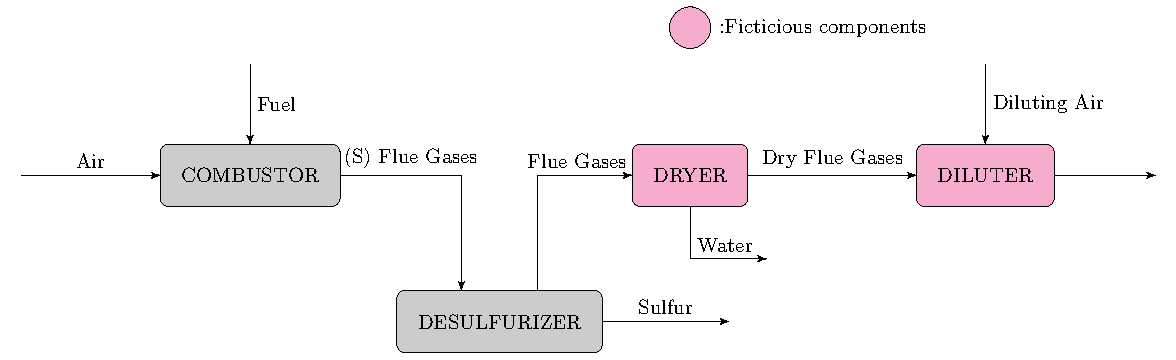
\includegraphics[width=\linewidth]{schemeB.pdf}
    \caption{Scheme of the theoretical model with desulfurizer.}
\end{figure}
%
We just need to introduce a step before the dryer.



\subparagraph*{From SULFURIZED FLUE GASES to FLUE GASES}
For the concentration of $\soo$ the equation that let to pass through the desulfurizer is equation number \ref{eq:SFG_FG_SO2}.
\begin{equation}
\label{eq:SFG_FG_SO2}
\chi_{\soo}^{\fg} = \chi_{\soo}^{\fgs} \cdot \frac{1 - \eta_{FGD}}{1 - \eta_{FGD} \cdot \chi_{\soo}^{\fgs}}
\end{equation}
where the coefficient $\displaystyle \frac{1 - \eta_{FGD}}{1 - \eta_{FGD} \cdot \chi_{\soo}^{\fgs}}$ is constant and equals to $\coefC$.
For any other substance the formula is slightly different because the $\soo$ molar flow rate changes passing through the desulfurizer while the mass and molar flow rates of the other molecules is constant. Therefore the correct equation is:
\begin{equation}
\label{eq:SFG_FGcoal}
\chi_{i}^{\fg} = \chi_{i}^{\fgs} \cdot \frac{1}{1 - \eta_{FGD} \cdot \chi_{\soo}^{\fgs}}
\end{equation}
where the coefficient $\displaystyle \frac{1}{1 - \eta_{FGD} \cdot \chi_{\soo}^{\fgs}}$ is constant and equals to $\coefD$.

The two following passages of the dryer and the diluter are exactly the same as the previous case. (Equations \ref{eq:FG_DFG} and \ref{eq:DFG_NORM})  



\subparagraph*{From FLUE GASES to DRY FLUE GASES}
\begin{equation}
\label{eq:FG_DFGcoal}
\chi_i^{\dfg} = \chi_i^{\fg} \cdot \frac{1}{1 - \chi_{\hoo}^{\fg}}
\end{equation}
We just miss $\chi_{\hoo}^{\fg}$ but we can get it with equation \ref{eq:SFG_FGcoal} applied for the water:
\begin{equation}
\chi_{\hoo}^{\dfg} = \chi_{\hoo}^{\fgs} / \coefD = \round{ 0.084815006040312*100}\perc
\end{equation}
The coefficient $\displaystyle \frac{1}{1 - \chi_{\hoo}^{\fg}}$ is constant and equals to $\coefAcoal$



\subparagraph*{From DRY FLUE GASES to NORMALIZED FLUE GASES}
\begin{equation}
\label{eq:DFG_NORMcoal}
\chi_i^{\norm} = \chi_i^{\dfg} \cdot \frac{\chi_{\oo}^{\norm} - \chi_{\hoo}^{\dil}}{\chi_{\oo}^{\dfg} - \chi_{\oo}^{\dil}}
\end{equation}
We just miss $\chi_{\oo}^{\fg}$ but we can get it with equations \ref{eq:SFG_FGcoal} \ref{eq:FG_DFGcoal} and  applied for the oxygen:
\begin{equation}
\chi_{\oo}^{\dfg} = \chi_{\oo}^{\fgs} / \coefAcoal / \coefD = \round{0.048199898122943*100}\perc
\end{equation}
%
The coefficient $\displaystyle \frac{\chi_{\oo}^{\norm} - \chi_{\hoo}^{\dil}}{\chi_{\oo}^{\dfg} - \chi_{\oo}^{\dil}}$ now can be calculated and it constant and equals to $\coefBcoal$.\\
The diluter is simply ambient air, with an oxygen concentration of $20.7\perc$.


\subsection{Absolute emission of $\nox$ as equivalent $\noo$}
We know the concentration of $\nox$ in dry flue gases with 3\% of $\oo$ so reverting equation \ref{eq:DFG_NORMcoal} we can get the concentration of $\nox$ in dry flue gases. From this value, using equation \ref{eq:FG_DFGcoal} we obtain their absolute concentration in flue gases that come out from the desulfurizer.


We know the concentration of $\nox$ in dry flue gases with 15\% of $\oo$ so reverting equation \ref{eq:DFG_NORMcoal} we can get the concentration of $\nox$ in dry flue gases. From this value, using equation \ref{eq:FG_DFGcoal} we obtain their absolute concentration in desulfurized flue gases. Finally we can pass from sulfurized flue gases to original flue gases with equation \ref{eq:SFG_FGcoal} instead of equation \ref{eq:SFG_FG_SO2} because we deal with emission of $\noo$. 

\begin{align}
\chi_{\noo}^{\fg}  &= (1 - \chi_{\hoo}^{\fg}) \cdot \chi_{\noo}^{\dfg} \\
				   &= (1 - \chi_{\hoo}^{\fg}) \cdot \frac{\chi_{\oo}^{\dfg} - \chi_{\oo}^{\dil}}
{\chi_{\oo}^{\norm} - \chi_{\hoo}^{\dil}} \cdot \chi_{\noo}^{\norm} \\
				   &= \dfrac{90\text{ ppmvd}}{ \coefAcoal \cdot \coefBcoal} 
= \round{8.89480655645772e-05*1000000}\E{-6}
\end{align}
The absolute emission of $\nox$ is computed as:
\begin{equation}
\label{eq:abs_emission_coal}
E_{i} \left[ \kgs \right] = \chi_i^{\fg} \cdot \MM{i} \cdot \ndot{\fg}
\end{equation}
From precept 1 we know that the mass flow rate of flue gases at the stack before desulfurizer is $\round{5.253457684875400e+02} \kgs$ and their mean molar mass is $\round{29.566436420120571}\kgkmols$. From these values we can evaluate the molar flow rate of flue gases as 
\begin{equation}
\ndot{\fg} = \frac{\mdot{\fg} }{ \MM{\fg}} = \round{17.768315431143110}\kmolss
\end{equation}
We are now able to compute the absolute emission of $\noo$.
\begin{equation}
E_{\noo} \left[ \kgs \right] = \chi_{\noo}^{\fg} \cdot \MM{\noo} \cdot \ndot{\fg}
 = \chi_{\noo}^{\fgs} \cdot \MM{\noo} \cdot \ndot{\fgs}
= \round{0.0725216067607346*1000}\E{-3} \kgs
\end{equation}

\subsection{$\nox$ mass concentration in dry flue gases}
With the conversion coefficient between flue gases and dry flue gases it is not so difficult to evaluate the concentration of $\noo$ in dry flue gases.
\begin{equation}
C_{\nox}^{\dfg} = \dfrac{\cancel{\ndot{\dfg}} \cdot \chi_{\noo}^{\dfg} \cdot \MM{\noo} \E{6} \mg / \kg }{\cancel{\ndot{\dfg}} \cdot 22.414}
= \round{199.469843922146} \left[ \frac{\mg_{\noo}}{Nm^3_{\dfg}} \right]
\end{equation}

\subsection{Absolute emission of $\coo$}
To evaluate absolute emission of $\coo$ we must apply equation \ref{eq:abs_emission_coal}.
\begin{equation}
E_{\coo} \left[ \kgs \right] = \chi_{\coo}^{\fg} \cdot \MM{\coo} \cdot \ndot{\fg}
= \round{99.2367757048432} \kgs
\end{equation}


\subsection{Concentration of $\soo$ in flue gases}
Concentration of $\soo$ must be compatible with legal limit of $200 \mg/Nm^3$ at 6\% of $\oo$.
To check the respect of this limit we must find the concentration of $soo$ in flue gases.

\begin{equation}
C_{\soo}^{\norm} = \dfrac{\cancel{\ndot{\norm}} \cdot \chi_{\soo}^{\norm} \cdot \MM{\soo} \E{6} \mg / \kg }{\cancel{\ndot{\norm}} \cdot 22.414}
\end{equation}

We miss the molar concentration of sulphur dioxide, but we know how to pass through the desulfurizer with equation \ref{eq:SFG_FG_SO2}

\begin{equation}
\chi_{\soo}^{\norm} = \chi_{\soo}^{\fgs} \cdot \frac{1 - \eta_{FGD}}{1 - \eta_{FGD} \cdot \chi_{\soo}^{\fgs}} 
\cdot \frac{1}{1 - \chi_{\hoo}^{\fg}}
\cdot \frac{\chi_{\oo}^{\norm} - \chi_{\hoo}^{\dil}}{\chi_{\oo}^{\dfg} - \chi_{\oo}^{\dil}}
 = \round{6.71862965766788e-05*1000000} \E{-6}
\end{equation}

So the final concentration of emitted $\soo$ is $C_{\soo}^{\fg} = \round{191.840946770208} \mgnmcube{\noo}{\dfg}$ that respect the legal limit of 200

\section{Natural gas combined cycle}
In	order	to	compare	the	emissions	of	the	steam	boilers	with	those	produced	by	the	NGCC,	it	is	necessary	to	compute	the	composition	of	the	flue	gas	at	the	combustor	outlet. From the net electric power and the total efficiency we can find the mass flow rate of fuel that we use to feed the combined cycle.
\begin{equation}
\eta_{CC} = \frac{\Wdot{net}}{\mdot{fuel} \cdot \text{LHV}} 
\qquad \Rightarrow \qquad
\mdot{fuel} = \frac{\Wdot{net}}{\eta_{CC} \cdot \text{LHV}} = \round{14.671050795742850} \kgs
\end{equation}
From the flue gases mass flow rate and the previous evaluated fuel mass flow rate we can get the air mass flow rate and consequentially also $\alpha$, the air over fuel mass ratio.
\begin{equation}
\mdot{air} = \mdot{flue\ gases} - \mdot{fuel} =\round{6.353289492042571e+02} \kgs
\end{equation}
\begin{equation}
\alpha = \frac{\mdot{air}}{\mdot{fuel}} = \round{43.304938279445722}
\end{equation}
We can write the chemical balance:
\begin{equation}
\label{chemical_balance}
\begin{split}
0.9\text{CH}_4 + 0.06\text{C}_2\text{H}_6 + 0.04\text{N}_2 + \beta_{O_2} \times
(O_2 + \frac{\chi_{\text{N}_2}}{\chi_{\text{O}_2}}\text{N}_2 + 
\frac{\chi_{\text{Ar}}}{\chi_{\text{O}_2}}\text{Ar} + \frac{\chi_{\text{H}_2\text{O}}}{\chi_{\text{O}_2}}\text{H}_2\text{O}
) = 
\\
a\text{CO}_2 + b\text{H}_2\text{O} + c\text{N}_2 + d\text{Ar} + e\text{O}_2
\end{split}
\end{equation}
We miss $\beta_{O_2}$ but we can obtain in from $\alpha$ previously evaluated.
\begin{equation}
\alpha
=\frac{\dot{m}_{AIR}}{\dot{m}_{fuel}}
=\beta_{\text{O}_2} \cdot \frac{1}{\chi_{\text{O}_2}^{air}} \cdot \frac{\text{MM}_{air}}{\text{MM}_{fuel}}
\end{equation}
\begin{equation}
\beta_{\text{O}_2} = \alpha \cdot \chi_{\text{O}_2}^{air} \cdot \frac{\text{MM}_{fuel}}{\text{MM}_{air}}
= \round{5.381427116382145}
\end{equation}
Balancing equation \ref{chemical_balance} we obtain the moles of chemical species in flue gases:
\begin{center}
\tabulinesep=1.2mm
$\begin{tabu}{|l|c|c|c|c|c|}
\hline
 & a\ (\text{CO}_2)  &  b\ (\text{H}_2\text{O})  &  c\ (\text{N}_2)  &  d\ (\text{Ar}) & e\ (\text{O}_2) \\ \hline
n & 1.02 & \round{2.247771494196793 } &  \round{20.135860680982599}  & \round{0.252173154729018} & \round{3.371427116382146
} 
 \\ \hline
\end{tabu}$
\end{center}
From that we easily get the concentration of each species in flue gases dividing the moles of each single species by the sum of all the species.
\begin{center}
\tabulinesep=1.2mm
$\begin{tabu}{|l|c|c|c|c|c|}
\hline
 & a\ (\text{CO}_2)  &  b\ (\text{H}_2\text{O})  &  c\ (\text{N}_2)  &  d\ (\text{Ar}) & e\ (\text{O}_2) \\ \hline
\chi & \round{0.037739713158829*100}\perc & \round{8.316691317409731 }\perc &  \round{74.502118265335795}\perc  & \round{0.933033580963739}\perc & \round{12.474185520407840} \perc
 \\ \hline
\end{tabu}$
\end{center}

A small	amount	of	nitrogen	does	not	bypass	the	combustion	but	it	oxidises	to	NOx, 14	ppmvd at $15\perc$ of $\oo$ ).	Yet,	we	can	neglect	its	presence	in	the	calculation	of	the	concentrations	of	the	other	products because it is really small for what that concern mass and energy, but it could be significant for environmental emission ($\chi_{\oo} \approx \round[round-precision=4]{15/1000000*100}\perc$).

To calculate the emission we use the same procedure of the natural gas case. 
\subsection{Absolute emission of $\nox$ as equivalent $\noo$}
\begin{equation}
\chi_{\noo}^{\fg} = (1 - \chi_{\hoo}^{\fg}) \cdot \frac{\chi_{\oo}^{\dfg} - \chi_{\oo}^{\dil}}
{\chi_{\oo}^{\norm} - \chi_{\hoo}^{\dil}} \cdot \chi_{\noo}^{\norm}
= \round{1.597537390814681e-05*1000000} \,\text{ppmvd}
\end{equation}
\begin{equation}
E_{\noo} \left[ \kgs \right] = \chi_{\noo}^{\fg} \cdot \MM{\noo} \cdot \ndot{\fg}
= \round{0.016829159537437*1000}\E{-3} \kgs
\end{equation}
\subsection{$\nox$ mass concentration in dry flue gases}
\begin{equation}
C_{\nox}^{\dfg} = \dfrac{\cancel{\ndot{\dfg}} \cdot \chi_{\noo}^{\dfg} \cdot \MM{\noo} \E{6} \mg / \kg }{\cancel{\ndot{\dfg}} \cdot 22.414}
= \round{32.786080118441745} \frac{\mg_{\noo}}{Nm^3_{\dfg}}
\end{equation}
\subsection{Absolute emission of $\coo$}
\begin{equation}
E_{\coo} \left[ \kgs \right] = \chi_{\coo}^{\fg} \cdot \MM{\coo} \cdot \ndot{\fg}
= \round{38.028118235560207} \kgs
\end{equation}
\subsection{Specific emission of $\nox$ per $\kwh$}
\begin{equation}
E_{\noo} \left[  \frac{\mg_{\noo}}{\kwh} \right] = \frac{\chi_{\noo}^{\fg} \cdot \MM{\noo} \cdot \ndot{\fg} \cdot 3600}{P_{\text{net}}^{\text{electric}}}
= \round{1.553460880378772e+02} \frac{\mg_{\noo}}{\kwh}
\end{equation}
\subsection{Specific emission of $\coo$ per $\kwh$}
\begin{equation}
E_{\coo} \left[  \frac{\g_{\coo}}{\kwh} \right] = \frac{\chi_{\coo}^{\fg} \cdot \MM{\coo} \cdot \ndot{\fg} \cdot 3600}{P_{\text{net}}^{\text{electric}}}
= \round{0.3510287837128635*1000} \frac{\g_{\coo}}{\kwh}
\end{equation}
\end{document}

